\documentclass[a1paper,portrait]{baposter}
\usepackage[utf8]{inputenc}
\usepackage{relsize}
\usepackage{amsmath,amsfonts,amssymb}

%%% Global Settings %%%%%%%%%%%%%%%%%%%%%%%%%%%%%%%%%%%%%%%%%%%%%%%%%%%%%%%%%%%

\graphicspath{{figures/}}	% Root directory of the pictures 

%%% Color Definitions %%%%%%%%%%%%%%%%%%%%%%%%%%%%%%%%%%%%%%%%%%%%%%%%%%%%%%%%%

\definecolor{bordercol}{RGB}{40,40,40}
\definecolor{headercol1}{RGB}{186,215,230}
\definecolor{headercol2}{RGB}{80,80,80}
\definecolor{headerfontcol}{RGB}{0,0,0}
\definecolor{boxcolor}{RGB}{186,215,230}
\definecolor{bgroundcol}{RGB}{245,245,245}

\begin{document}
\begin{poster}{
		grid=false,
		eyecatcher=false,
		columns=2,
		borderColor=bordercol,
		headerColorOne=headercol1,
		headerColorTwo=headercol2,
		headerFontColor=headerfontcol,
		boxColorOne=boxcolor,
		headershape=roundedright,
		textborder=faded,
		background=plain,
		bgColorOne=bgroundcol,
		headerborder=open,
		boxshade=plain,
}
{
	% Eye catcher
}
%% Title
{\sf\bf
	Restricted Boltzmann Machine\\
	{\vspace{0.5em}\Large A Probabilistic Graphical Model course's project}
}
%% Authors
{
	Chaïmaa Kadaoui, Othman Sbai, Xi Shen
}
%% Logo
{
	
\includegraphics[width=10em]{Logo}
}

\headerbox{Definition}{name=definition,column=0, row=0}{
\smaller
A Restricted Boltzman Machine is an undirected graph which can be decomposed in two layers.


\includegraphics[width=\linewidth]{rbm}

It is \emph{restricted} because no connection between nodes of the same layer is supposed. The matrix $W$ characterizes the connections between the two layers. For simplification, we suppose that the variables $ \mathbf{x} $ and $ \mathbf{h} $ are binary.
}

\headerbox{Energy and probability}{name=energy,column=1, row=0}{
\smaller
We introduce the two bias vectors $c$ and $b$ to define the energy of this graph:

\[ E(x,h) = -h^\top W x - c^\top x - b^\top h \]

We can write the joint probability of $ \mathbf{x} $ and $ \mathbf{h} $ as: 

\[ p(x,h) = \exp(-E(x,h)) / Z \]

$Z$ is the partition parameter which can be computed by calculating all the possibles values of $ \mathbf{x} $  and $ \mathbf{h} $ . In practice, this parameter is intractable. 

\textbf{Inference} We can prove that given $\mathbf{x}$, $h_j$ follows a Bernoulli: $$p(h_j=1|x) = sigm(b_j + W_{j.}x)$$
$ W_{j.}$ is the j-th row of $W$ and $sigm$ defines the sigmoid function.
}

\headerbox{Contrastive Divergence}{name=CD,column=0, below=definition, span=2}{
\smaller
To train the RBM with our data $\mathbf{x}^{(t)}$, we would like to minimize the average loss:
$ \frac{1}{T} \sum_t l(f(\mathbf{x}^{(t)})) =  \frac{1}{T} \sum_t - \log p(\mathbf{x}^{(t)}) $

We will apply a stochastic gradient descent. We derive each term of the sum with respect to our model parameter $\theta$ as follow (where $\mathbb{E}_h$ and $\mathbb{E}_{x,h}$ are expectations of $h$ and $(x,h)$ respectively):

\[ \frac{\partial - \log p(\mathbf{x}^{(t)})}{\partial \theta} = \mathbb{E}_h \left[ \frac{\partial E(\mathbf{x}^{(t)} ,h)}{\partial \theta} | \mathbf{x}^{(t)} \right] - \mathbb{E}_{x,h} \left[ \frac{\partial E(\mathbf{x} ,h)}{\partial \theta} \right] \]

The first term is called the \emph{positive phase} and the second term the \emph{negative phase}. Because of the difficulty to compute the seconde term, we will use an algorithm called \emph{Contrastive Divergence}. The key points of the algorithm are:

\begin{itemize}
	\itemsep=-0.02em
	\item We estimate the expectation $\mathbb{E}_{x,h}$ by sampling a single point $\mathbf{\tilde x}$.
	\item To do so, we use Gibbs sampling in chain (we apply it $k$ times).
	\item We initialize our Gibbs sampling with $\mathbf{x^{(t)}}$.
\end{itemize}

}

\headerbox{Results}{name=results,column=0, below=CD}{
\smaller
We implemented the algorithm and applied it to the MNIST dataset.

	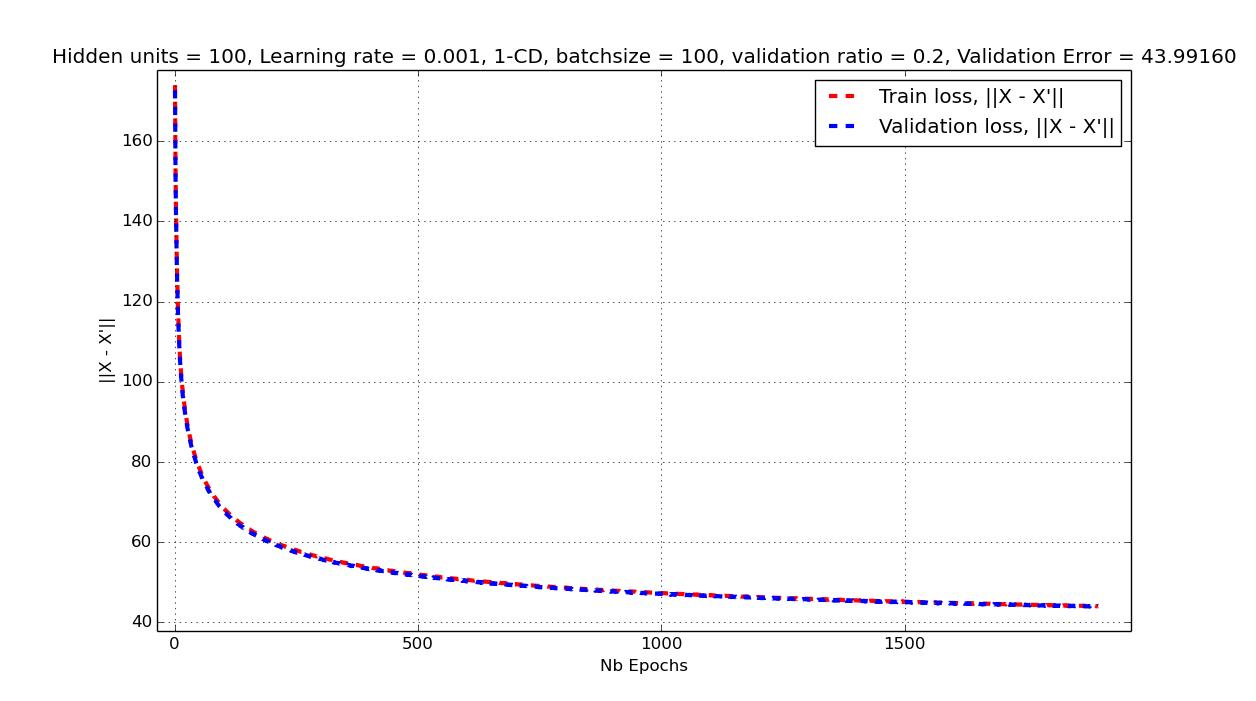
\includegraphics[width=\linewidth]{TrainCurve}
}
\headerbox{Interpretation}{name=interpretation,column=1, below=CD}{
	
}

\headerbox{References}{name=refs,column=0, below=results, span=2}{
\smaller													
\vspace{-0.4em} 										
\bibliographystyle{plain}						
\renewcommand{\section}[2]{\vskip 0.05em}
\begin{thebibliography}{1}						
	\itemsep=-0.01em									
	\setlength{\baselineskip}{0.4em}				
	\bibitem{praticalGuide} Hinton G. \textit{ A practical guide to training restricted Boltzmann machines[J]. Momentum, 2010, 9(1): 926.}
	\bibitem{these} Fischer A. \textit{Training restricted boltzmann machines[J]. KI-Künstliche Intelligenz, 2015, 29(4): 441-444.}
	\bibitem{reviewArticle} Bengio, Y., Delalleau, O. \textit{Justifying and generalizing contrastive divergence}. Neural Computation 21(6), 1601n621 (2009)
\end{thebibliography}
}


	
\end{poster}
\end{document}